\documentclass[12pt,a4paper,oneside]{report}
\newif\ifchronologia
\ifdefined\Chronologia\chronologiatrue\else\chronologiafalse\fi

% Typografia wzorowana na „Miara i całka” G. Plebanka:
% PL Roman, 12 pt, A4, klasyczne rozdziały i podrozdziały.
\usepackage[utf8]{inputenc}
\usepackage[OT4,plmath]{polski}
\usepackage{amsmath,amssymb,amsthm}
\usepackage[left=30.56mm,right=26.2mm,top=30mm,bottom=28mm]{geometry}
\usepackage{microtype}
\usepackage{graphicx}
\usepackage{eso-pic}
\usepackage{enumitem}
\usepackage[hidelinks,unicode]{hyperref}

\hypersetup{
  pdftitle={Teoria miary},
  pdfsubject={Skrypt z wykładów},
  linktoc=all,
  bookmarksnumbered=true
}
\graphicspath{{../grafika/}}
\setcounter{tocdepth}{1}
\setcounter{secnumdepth}{2}
\setlength{\parindent}{1.5em}
\setlength{\parskip}{0pt}
\setlist[enumerate]{label=\arabic*),leftmargin=2.1em,itemsep=0.25em}
\allowdisplaybreaks[1]
% Zachowaj numer rozdziału także przy wzorach w rozdziale 0.
\renewcommand{\theequation}{\thechapter.\arabic{equation}}

\theoremstyle{definition}
% Każdy rodzaj ma osobny licznik, ciągły przez cały rozdział.
\newtheorem{definicja}{Definicja}[chapter]
\newtheorem{przyklad}{Przykład}[chapter]
\newtheorem{uwaga}{Uwaga}[chapter]
\theoremstyle{plain}
\newtheorem{fakt}{Fakt}[chapter]
\newtheorem{twierdzenie}{Twierdzenie}[chapter]
\newtheorem{lemat}{Lemat}[chapter]
\newtheorem{wniosek}{Wniosek}[chapter]
\renewcommand{\proofname}{Dowód}

% Znaczniki nie zmieniają rozdziałów, sekcji ani liczników matematycznych.
\newcommand{\poczatekwykladu}[1]{%
  \ifchronologia
    \par\addvspace{\baselineskip}%
    \phantomsection
    \addcontentsline{toc}{section}{Wykład #1}%
    \noindent{\large\bfseries Wykład #1}\par\nobreak
    \noindent\rule{\linewidth}{0.4pt}\par\nobreak
    \addvspace{0.5\baselineskip}%
  \fi
}

% Limbo jest widoczne w obu wariantach i nie zmienia numeracji.
\newcommand{\znaczniklimbo}{%
  \par\addvspace{\baselineskip}%
  \phantomsection
  \addcontentsline{toc}{section}{Limbo}%
  \noindent{\large\bfseries Limbo}\par\nobreak
  \noindent\rule{\linewidth}{0.4pt}\par\nobreak
  \addvspace{0.5\baselineskip}%
}

\newcommand{\R}{\mathbb{R}}
\newcommand{\N}{\mathbb{N}}
\newcommand{\A}{\mathcal{A}}
\newcommand{\Rbar}{\overline{\mathbb{R}}}



\begin{document}

\hypersetup{pageanchor=false}
% Wspólna okładka, potem strona tytułowa przed spisem treści.
\begin{titlepage}
  \thispagestyle{empty}
  \AddToShipoutPictureBG*{%
    \AtPageLowerLeft{%
      \pdfximage width\paperwidth height\paperheight {../grafika/okladka.pdf}%
      \pdfrefximage\pdflastximage
    }%
  }
  \null
\end{titlepage}

\begin{titlepage}
  \thispagestyle{empty}
  \centering
  \vspace*{\fill}
  {\LARGE\bfseries Teoria miary\par}
  \vspace{0.7cm}
  {\large Skrypt z wykładów\par}
  \vspace{0.35cm}
  \ifchronologia
    {\normalsize Z oznaczeniem chronologii wykładu\par}
  \else
    {\normalsize Bez oznaczenia chronologii wykładu\par}
  \fi
  \vspace{1.3cm}
  {\large Opracowanie: Szymon Gaziński\par}
  \vspace*{\fill}
\end{titlepage}


\pagenumbering{roman}
\hypersetup{pageanchor=true}
\pdfbookmark[0]{Spis treści}{spis-tresci}
\tableofcontents
\clearpage
\pagenumbering{arabic}
\pagestyle{plain}

\setcounter{chapter}{-1}
\chapter{Podstawowe pojęcia}
\label{chap:podstawowe-pojecia}
\poczatekwykladu{1}

\section{Odcinki i prostokąty}
\label{sec:terminologia}

\begin{definicja}[Odcinki]
Niech $a,b\in\R$ oraz $a\leq b$. Odcinek otwarty o końcach $a$ i $b$ to
\begin{equation}
  (a,b)=\{x\in\R:a<x<b\}.
  \label{eq:odcinek-otwarty}
\end{equation}
Analogicznie określamy odcinek domknięty i odcinki półotwarte:
\begin{align*}
  [a,b]&=\{x\in\R:a\leq x\leq b\},\\
  [a,b)&=\{x\in\R:a\leq x<b\},\\
  (a,b]&=\{x\in\R:a<x\leq b\}.
\end{align*}
W szczególności jednopunktowy zbiór $\{a\}$ zapisujemy również jako $[a,a]$.
\end{definicja}

\begin{definicja}[Prostokąt uogólniony]
Niech $d\in\N$ oraz niech $I_1,\ldots,I_d$ będą odcinkami w $\R$.
Prostokątem uogólnionym w $\R^d$ nazywamy zbiór
\begin{equation}
  P=I_1\times\cdots\times I_d
   =\{(x_1,\ldots,x_d)\in\R^d:
       x_i\in I_i\text{ dla każdego }i=1,\ldots,d\}.
  \label{eq:prostokat}
\end{equation}
\end{definicja}

\section{Prosta rozszerzona}
\label{sec:prosta-rozszerzona}

\begin{definicja}[Prosta rozszerzona]
Prostą rozszerzoną nazywamy zbiór
\begin{equation}
  \Rbar=[-\infty,+\infty]=\R\cup\{-\infty,+\infty\}.
  \label{eq:prosta-rozszerzona}
\end{equation}
Dla każdej liczby $a\in\R$ przyjmujemy
\[
  -\infty<a<+\infty.
\]
\end{definicja}

Dla $a\in\R$ obowiązują reguły
\begin{align*}
  a+(+\infty)&=(+\infty)+a=+\infty,\\
  a-(+\infty)&=-\infty.
\end{align*}
W teorii miary stosujemy także konwencję
\begin{equation}
  0\cdot(+\infty)=(+\infty)\cdot0=0.
  \label{eq:zero-nieskonczonosc}
\end{equation}

\begin{uwaga}
Równość \eqref{eq:zero-nieskonczonosc} jest przyjętą konwencją rachunku
na prostej rozszerzonej. Nie jest regułą obliczania granic: iloczyn typu
$0\cdot\infty$ w zadaniu o granicach pozostaje formą nieoznaczoną.
\end{uwaga}

\section{Granica górna i dolna ciągu zbiorów}
\label{sec:granice-zbiorow}

Niech $(A_n)_{n\geq1}$ będzie ciągiem podzbiorów ustalonego zbioru $X$.

\begin{definicja}[Granica górna]
Granicą górną ciągu $(A_n)$ nazywamy zbiór
\begin{equation}
  \limsup_{n\to\infty}A_n
  =\bigcap_{n=1}^{\infty}\bigcup_{k=n}^{\infty}A_k
  =\{x\in X:\forall n\geq1\ \exists k\geq n\quad x\in A_k\}.
  \label{eq:limsup}
\end{equation}
Innymi słowy, $x\in\limsup_{n\to\infty}A_n$ wtedy i tylko wtedy, gdy $x$
należy do nieskończenie wielu zbiorów $A_n$.
\end{definicja}

\begin{definicja}[Granica dolna]
Granicą dolną ciągu $(A_n)$ nazywamy zbiór
\begin{equation}
  \liminf_{n\to\infty}A_n
  =\bigcup_{n=1}^{\infty}\bigcap_{k=n}^{\infty}A_k
  =\{x\in X:\exists n\geq1\ \forall k\geq n\quad x\in A_k\}.
  \label{eq:liminf}
\end{equation}
Innymi słowy, $x\in\liminf_{n\to\infty}A_n$ wtedy i tylko wtedy, gdy $x$
należy do prawie wszystkich zbiorów $A_n$, czyli do wszystkich od pewnego
miejsca ciągu.
\end{definicja}

\begin{fakt}
Dla każdego ciągu zbiorów $(A_n)$ zachodzi
\begin{equation}
  \liminf_{n\to\infty}A_n\subseteq\limsup_{n\to\infty}A_n.
  \label{eq:inkluzja-granic}
\end{equation}
\end{fakt}

\begin{proof}
Jeżeli punkt należy do wszystkich zbiorów od pewnego miejsca ciągu,
to należy do nieskończenie wielu zbiorów tego ciągu.
\end{proof}

\begin{definicja}[Zbieżność ciągu zbiorów]
Jeżeli
\[
  \liminf_{n\to\infty}A_n=\limsup_{n\to\infty}A_n,
\]
to mówimy, że ciąg $(A_n)$ jest zbieżny. Wspólną wartość tych granic
oznaczamy przez $\lim_{n\to\infty}A_n$.
\end{definicja}

\section{Przykłady granic ciągów zbiorów}
\label{sec:przyklady-granic}

\begin{przyklad}[Ciąg naprzemienny]
Niech
\[
  A_n=[0,1+(-1)^n],\qquad n\geq1.
\]
Wówczas
\[
  A_{2k-1}=\{0\},\qquad A_{2k}=[0,2],\qquad k\geq1.
\]
Punkt $0$ należy do każdego zbioru $A_n$. Każdy punkt $x\in(0,2]$ należy
do wszystkich zbiorów o indeksach parzystych, a nie należy do żadnego
zbioru o indeksie nieparzystym. Punkty spoza $[0,2]$ nie należą do
żadnego z tych zbiorów. Zatem, zgodnie z \eqref{eq:limsup} i \eqref{eq:liminf},
\begin{equation}
  \liminf_{n\to\infty}A_n=\{0\},\qquad
  \limsup_{n\to\infty}A_n=[0,2].
  \label{eq:przyklad-naprzemienny}
\end{equation}
Granice są różne, więc ciąg $(A_n)$ nie jest zbieżny.
\end{przyklad}

\begin{przyklad}[Początkowe odcinki zbioru liczb naturalnych]
Przyjmujemy $\N=\{1,2,3,\ldots\}$ i rozważamy ciąg
\[
  A_n=\{1,2,\ldots,n\},\qquad n\geq1.
\]
Dla każdego $m\in\N$ mamy $m\in A_n$ dla wszystkich $n\geq m$.
Każda liczba naturalna należy więc do prawie wszystkich zbiorów $A_n$.
Punkty spoza $\N$ nie należą do żadnego z nich. Stąd
\begin{equation}
  \liminf_{n\to\infty}A_n=\N=\limsup_{n\to\infty}A_n,
  \qquad \lim_{n\to\infty}A_n=\N.
  \label{eq:przyklad-naturalne}
\end{equation}
\end{przyklad}

\chapter{Struktury na zbiorach}
\label{chap:cialo-pierscien-przestrzen-mierzalna}

\section{Ciało i sigma-ciało zbiorów}
\label{sec:cialo-sigma-cialo}

\begin{definicja}[Ciało zbiorów]
\label{def:cialo}
Ciałem zbiorów w przestrzeni $X$ nazywamy rodzinę $\A\subseteq\mathcal{P}(X)$
spełniającą następujące warunki:
\begin{enumerate}
  \item $\varnothing\in\A$;
  \item jeżeli $A,B\in\A$, to $A\cup B\in\A$;
  \item jeżeli $A\in\A$, to $A^c\in\A$, gdzie $A^c=X\setminus A$.
\end{enumerate}
\end{definicja}

\begin{definicja}[Sigma-ciało zbiorów]
\label{def:sigma-cialo}
Sigma-ciałem (\mbox{$\sigma$-ciałem}) zbiorów w przestrzeni $X$ nazywamy
rodzinę $\A\subseteq\mathcal{P}(X)$, dla której warunki 1) i 3) z definicji
ciała są zachowane, a warunek 2) zastępujemy warunkiem:
\begin{enumerate}[label=2\textquotesingle),start=2]
  \item jeżeli $A_n\in\A$ dla każdego $n\geq1$, to
  \[
    \bigcup_{n=1}^{\infty}A_n\in\A.
  \]
\end{enumerate}
\end{definicja}

\poczatekwykladu{2}
\section{Własności sigma-ciał}
\label{sec:wlasnosci-sigma-cial}

Niech $\A$ będzie sigma-ciałem podzbiorów zbioru $X$.
Wszystkie dopełnienia w tej części rozumiemy względem $X$.

\begin{fakt}
Zbiór $X$ należy do $\A$.
\end{fakt}

\begin{proof}
Mamy $\varnothing\in\A$, a rodzina $\A$ jest zamknięta na dopełnienia.
Zatem $X=\varnothing^c\in\A$.
\end{proof}

\begin{fakt}[Skończone sumy]
Jeżeli $A_1,\ldots,A_m\in\A$, to
\[
  \bigcup_{k=1}^{m}A_k\in\A.
\]
\end{fakt}

\begin{proof}
Połóżmy $A_k=\varnothing$ dla $k>m$. Wtedy wszystkie zbiory tego ciągu
należą do $\A$ i
\[
  \bigcup_{k=1}^{m}A_k=\bigcup_{k=1}^{\infty}A_k\in\A.
\]
\end{proof}

\begin{fakt}[Przeliczalne i skończone przekroje]
Jeżeli $A_n\in\A$ dla każdego $n\geq1$, to
\[
  \bigcap_{n=1}^{\infty}A_n\in\A.
\]
Rodzina $\A$ jest również zamknięta na skończone przekroje.
\end{fakt}

\begin{proof}
Z praw de Morgana otrzymujemy
\begin{equation}
  \bigcap_{n=1}^{\infty}A_n
  =\left(\bigcup_{n=1}^{\infty}A_n^c\right)^c\in\A.
  \label{eq:przekroj-de-morgan}
\end{equation}
Skończone przekroje otrzymujemy tak samo, stosując prawo de Morgana
do skończonych sum.
\end{proof}

\begin{fakt}[Różnice zbiorów]
Jeżeli $A,B\in\A$, to $A\setminus B\in\A$.
\end{fakt}

\begin{proof}
Wystarczy skorzystać z równości $A\setminus B=A\cap B^c$.
\end{proof}

\begin{fakt}[Różnice symetryczne]
Jeżeli $A,B\in\A$, to $A\mathbin{\triangle}B\in\A$, gdzie
\[
  A\mathbin{\triangle}B=(A\setminus B)\cup(B\setminus A).
\]
\end{fakt}

\begin{proof}
Oba zbiory $A\setminus B$ i $B\setminus A$ należą do $\A$, a rodzina
$\A$ jest zamknięta na sumy dwóch zbiorów.
\end{proof}

\begin{uwaga}[Równoważna postać definicji sigma-ciała]
W definicji sigma-ciała wystarczy założyć, że rodzina $\A$ jest niepusta
oraz zamknięta na dopełnienia i przeliczalne sumy.
Warunek $\varnothing\in\A$ wynika wtedy z pozostałych założeń.
\end{uwaga}

\begin{proof}
Wybierzmy $A\in\A$. Wtedy $A^c\in\A$ oraz
$X=A\cup A^c\in\A$ (sumę dwóch zbiorów można zapisać jako sumę
przeliczalną, powtarzając je w ciągu). Stąd $\varnothing=X^c\in\A$.
\end{proof}

\section{Zbiory przeliczalne i ich dopełnienia}
\label{sec:przeliczalne-dopelnienia}

\begin{przyklad}
Niech $X$ będzie dowolnym zbiorem. Rodzina
\begin{equation}
  \A=\{A\subseteq X:
    A\text{ jest przeliczalny lub }A^c\text{ jest przeliczalny}\}
  \label{eq:sigma-cialo-przeliczalne}
\end{equation}
jest sigma-ciałem. Przez zbiór przeliczalny rozumiemy tutaj także zbiór
skończony, czyli zbiór o mocy nie większej niż $\aleph_0$.
\end{przyklad}

\begin{proof}
Sprawdzamy trzy warunki z definicji~\ref{def:sigma-cialo}.
\begin{enumerate}
  \item Zbiór $\varnothing$ jest przeliczalny, więc $\varnothing\in\A$.
  \item Niech $A\in\A$ i $B=A^c$. Jeżeli $A$ jest przeliczalny,
  to $B^c=A$ jest przeliczalny. Jeżeli $A^c$ jest przeliczalny,
  to przeliczalny jest sam zbiór $B$. W obu przypadkach $B=A^c\in\A$.
  \item Niech $A_n\in\A$ dla każdego $n\geq1$. Rozważamy dwa przypadki.

  Jeżeli wszystkie zbiory $A_n$ są przeliczalne, to ich przeliczalna suma
  $\bigcup_{n=1}^{\infty}A_n$ jest przeliczalna, zatem należy do $\A$.

  Jeżeli pewien zbiór $A_{n_0}$ nie jest przeliczalny, to z $A_{n_0}\in\A$
  wynika, że $A_{n_0}^c$ jest przeliczalny. Ponadto
  \begin{equation}
    \left(\bigcup_{n=1}^{\infty}A_n\right)^c
    =\bigcap_{n=1}^{\infty}A_n^c\subseteq A_{n_0}^c.
    \label{eq:dopelnienie-sumy-przeliczalne}
  \end{equation}
  Dopełnienie sumy jest więc przeliczalne. W tym przypadku również
  $\bigcup_{n=1}^{\infty}A_n\in\A$.
\end{enumerate}
\end{proof}

\section{Przestrzeń mierzalna}
\label{sec:przestrzen-mierzalna}

\begin{definicja}[Przestrzeń mierzalna]
Przestrzenią mierzalną nazywamy parę $(X,\mathcal{F})$, gdzie
$\mathcal{F}$ jest sigma-ciałem podzbiorów zbioru $X$.
\end{definicja}

\section{Przekroje i sigma-ciała generowane}
\label{sec:sigma-ciala-generowane}

\begin{twierdzenie}[Przekrój sigma-ciał]
Niech $(\mathcal{F}_t)_{t\in T}$ będzie rodziną sigma-ciał podzbiorów
ustalonego zbioru $X$. Wówczas
\begin{equation}
  \mathcal{G}=\bigcap_{t\in T}\mathcal{F}_t
  \label{eq:przekroj-sigma-cial}
\end{equation}
jest sigma-ciałem. Dla pustej rodziny przyjmujemy, że jej przekrój
jest równy $\mathcal{P}(X)$.
\label{tw:przekroj-sigma-cial}
\end{twierdzenie}

\begin{proof}
Jeżeli $T=\varnothing$, to $\mathcal{G}=\mathcal{P}(X)$ jest sigma-ciałem.
Załóżmy zatem, że $T\neq\varnothing$.
\begin{enumerate}
  \item Dla każdego $t\in T$ mamy $\varnothing\in\mathcal{F}_t$,
  więc $\varnothing\in\mathcal{G}$.
  \item Jeżeli $A_n\in\mathcal{G}$ dla każdego $n\geq1$, to dla każdego
  $t\in T$ wszystkie zbiory $A_n$ należą do $\mathcal{F}_t$.
  Zatem dla każdego $t\in T$ mamy
  \[
    \bigcup_{n=1}^{\infty}A_n\in\mathcal{F}_t,
  \]
  czyli $\bigcup_{n=1}^{\infty}A_n\in\mathcal{G}$.
  \item Jeżeli $A\in\mathcal{G}$, to $A\in\mathcal{F}_t$ dla każdego
  $t\in T$. Stąd $A^c\in\mathcal{F}_t$ dla każdego $t\in T$,
  a więc $A^c\in\mathcal{G}$.
\end{enumerate}
\end{proof}

\begin{wniosek}
Dla dowolnej rodziny $\mathcal{E}\subseteq\mathcal{P}(X)$ istnieje
najmniejsze, w sensie zawierania, sigma-ciało podzbiorów $X$
zawierające $\mathcal{E}$.
\label{wn:najmniejsze-sigma-cialo}
\end{wniosek}

\begin{proof}
Rozważmy rodzinę wszystkich sigma-ciał zawierających $\mathcal{E}$:
\[
  \mathfrak{S}=\{\mathcal{F}\subseteq\mathcal{P}(X):
    \mathcal{F}\text{ jest sigma-ciałem i }\mathcal{E}\subseteq\mathcal{F}\}.
\]
Rodzina $\mathfrak{S}$ jest niepusta, ponieważ należy do niej
$\mathcal{P}(X)$. Z twierdzenia~\ref{tw:przekroj-sigma-cial} wynika, że
\[
  \mathcal{G}=\bigcap_{\mathcal{F}\in\mathfrak{S}}\mathcal{F}
\]
jest sigma-ciałem. Każdy element $\mathcal{E}$ należy do każdego
$\mathcal{F}\in\mathfrak{S}$, zatem $\mathcal{E}\subseteq\mathcal{G}$.
Jeżeli $\mathcal{F}_0$ jest dowolnym sigma-ciałem zawierającym
$\mathcal{E}$, to $\mathcal{F}_0\in\mathfrak{S}$, więc
$\mathcal{G}\subseteq\mathcal{F}_0$.
\end{proof}

\begin{definicja}[Sigma-ciało generowane]
Najmniejsze sigma-ciało zawierające rodzinę
$\mathcal{E}\subseteq\mathcal{P}(X)$ nazywamy sigma-ciałem
generowanym przez $\mathcal{E}$ i oznaczamy przez $\sigma(\mathcal{E})$.
Zatem
\begin{equation}
  \sigma(\mathcal{E})
  =\bigcap\{\mathcal{F}:\mathcal{F}\text{ jest sigma-ciałem w }X,
     \ \mathcal{E}\subseteq\mathcal{F}\}.
  \label{eq:sigma-generowane}
\end{equation}
\end{definicja}

\section{Sigma-ciało zbiorów borelowskich}
\label{sec:zbiory-borelowskie}

\begin{definicja}[Zbiory borelowskie na prostej]
Sigma-ciało generowane przez wszystkie zbiory otwarte w $\R$
nazywamy sigma-ciałem zbiorów borelowskich i oznaczamy przez
$\mathcal{B}(\R)$. Jego elementy nazywamy zbiorami borelowskimi.
\end{definicja}

\begin{fakt}
Sigma-ciało $\mathcal{B}(\R)$ jest generowane przez rodzinę wszystkich
odcinków otwartych:
\begin{equation}
  \mathcal{B}(\R)
  =\sigma\bigl(\{(a,b):a,b\in\R,\ a<b\}\bigr).
  \label{eq:borel-odcinki}
\end{equation}
\end{fakt}

\begin{proof}
Każdy odcinek otwarty jest zbiorem otwartym, zatem sigma-ciało po prawej
stronie \eqref{eq:borel-odcinki} zawiera się w $\mathcal{B}(\R)$.
Z drugiej strony każdy zbiór otwarty $U\subseteq\R$ jest sumą wszystkich
odcinków $(p,q)\subseteq U$ o wymiernych końcach $p<q$.
Takich odcinków jest co najwyżej przeliczalnie wiele. Zatem każdy zbiór
otwarty należy do sigma-ciała generowanego przez odcinki otwarte,
co daje przeciwną inkluzję.
\end{proof}

\begin{uwaga}
Sama rodzina $\mathcal{J}$ wszystkich odcinków nie jest sigma-ciałem.
Na przykład $(0,1)\in\mathcal{J}$, ale jego dopełnienie w $\R$,
\[
  (0,1)^c=(-\infty,0]\cup[1,+\infty),
\]
nie jest odcinkiem, więc nie należy do $\mathcal{J}$.
\end{uwaga}

\begin{samepage}
\section{Pierścienie i sigma-pierścienie zbiorów}
\label{sec:pierscienie}

\begin{definicja}[Pierścień zbiorów]
Pierścieniem zbiorów w $X$ nazywamy rodzinę
$\mathcal{R}\subseteq\mathcal{P}(X)$ spełniającą warunki:
\begin{enumerate}
  \item $\varnothing\in\mathcal{R}$;
  \item jeżeli $A,B\in\mathcal{R}$, to $A\cup B\in\mathcal{R}$;
  \item jeżeli $A,B\in\mathcal{R}$, to $A\setminus B\in\mathcal{R}$.
\end{enumerate}
\end{definicja}

\begin{definicja}[Sigma-pierścień zbiorów]
Sigma-pierścieniem zbiorów w $X$ nazywamy pierścień
$\mathcal{R}\subseteq\mathcal{P}(X)$ zamknięty na przeliczalne sumy.
Oznacza to, że warunek 2) w definicji pierścienia zastępujemy warunkiem:
jeżeli $A_n\in\mathcal{R}$ dla każdego $n\geq1$, to
\[
  \bigcup_{n=1}^{\infty}A_n\in\mathcal{R}.
\]
\end{definicja}
\end{samepage}

\poczatekwykladu{3}
\section{Ideały i filtry zbiorów}
\label{sec:idealy-filtry}

W tej części wszystkie rozważane zbiory są podzbiorami ustalonego zbioru
$X$, a dopełnienia bierzemy względem $X$.

\begin{definicja}[Ideał zbiorów]
\label{def:ideal}
Rodzinę $\mathcal{I}\subseteq\mathcal{P}(X)$ nazywamy ideałem zbiorów,
jeżeli spełnia następujące warunki:
\begin{enumerate}
  \item $\varnothing\in\mathcal{I}$ oraz $X\notin\mathcal{I}$;
  \item jeżeli $A,B\in\mathcal{I}$, to $A\cup B\in\mathcal{I}$;
  \item jeżeli $A\subseteq B$ i $B\in\mathcal{I}$, to $A\in\mathcal{I}$.
\end{enumerate}
Ostatni warunek oznacza, że każdy podzbiór elementu ideału również
należy do tego ideału.
\end{definicja}

\begin{przyklad}[Ideał zbiorów skończonych]
\label{prz:ideal-skonczone}
Dla $X=\R$ rodzina
\begin{equation}
  \mathcal{I}_{\mathrm{fin}}
  =\{A\subseteq\R:A\text{ jest skończony}\}
  \label{eq:ideal-skonczone}
\end{equation}
jest ideałem zbiorów.
\end{przyklad}

\begin{proof}
Sprawdzamy kolejno warunki definicji~\ref{def:ideal}.
\begin{enumerate}
  \item Zbiór pusty jest skończony, więc
  $\varnothing\in\mathcal{I}_{\mathrm{fin}}$.
  Zbiór $\R$ jest nieskończony, zatem $\R\notin\mathcal{I}_{\mathrm{fin}}$.
  \item Jeżeli $A,B\in\mathcal{I}_{\mathrm{fin}}$, to oba zbiory są
  skończone. Ich suma jest skończona, gdyż
  $|A\cup B|\leq|A|+|B|<\infty$.
  Stąd $A\cup B\in\mathcal{I}_{\mathrm{fin}}$.
  \item Jeżeli $A\subseteq B$ i $B\in\mathcal{I}_{\mathrm{fin}}$,
  to $|A|\leq|B|<\infty$. Zatem $A$ jest skończony i należy
  do $\mathcal{I}_{\mathrm{fin}}$.
\end{enumerate}
\end{proof}

\begin{definicja}[Filtr zbiorów]
\label{def:filtr}
Rodzinę $\mathcal{F}\subseteq\mathcal{P}(X)$ nazywamy filtrem zbiorów,
jeżeli spełnia następujące warunki:
\begin{enumerate}
  \item $X\in\mathcal{F}$ oraz $\varnothing\notin\mathcal{F}$;
  \item jeżeli $A,B\in\mathcal{F}$, to $A\cap B\in\mathcal{F}$;
  \item jeżeli $A\subseteq B\subseteq X$ i $A\in\mathcal{F}$,
  to $B\in\mathcal{F}$.
\end{enumerate}
Ostatni warunek oznacza, że każdy nadzbiór elementu filtru, zawarty
w $X$, również należy do tego filtru.
\end{definicja}

\begin{przyklad}[Filtr zbiorów o skończonym dopełnieniu]
\label{prz:filtr-dopelnienia-skonczone}
Dla $X=\R$ rodzina
\begin{equation}
  \mathcal{F}_{\mathrm{cofin}}
  =\{A\subseteq\R:A^c\text{ jest skończony}\}
  \label{eq:filtr-dopelnienia-skonczone}
\end{equation}
jest filtrem zbiorów.
\end{przyklad}

\begin{proof}
Sprawdzamy kolejno warunki definicji~\ref{def:filtr}.
\begin{enumerate}
  \item Mamy $\R^c=\varnothing$, więc
  $\R\in\mathcal{F}_{\mathrm{cofin}}$.
  Natomiast $\varnothing^c=\R$ jest nieskończony, zatem
  $\varnothing\notin\mathcal{F}_{\mathrm{cofin}}$.
  \item Jeżeli $A,B\in\mathcal{F}_{\mathrm{cofin}}$, to
  $A^c$ i $B^c$ są skończone. Z prawa de Morgana otrzymujemy
  \[
    (A\cap B)^c=A^c\cup B^c.
  \]
  Prawa strona jest sumą dwóch zbiorów skończonych, więc jest skończona.
  Stąd $A\cap B\in\mathcal{F}_{\mathrm{cofin}}$.
  \item Jeżeli $A\subseteq B\subseteq\R$ i
  $A\in\mathcal{F}_{\mathrm{cofin}}$, to $B^c\subseteq A^c$.
  Ponieważ $A^c$ jest skończony, również $B^c$ jest skończony.
  Zatem $B\in\mathcal{F}_{\mathrm{cofin}}$.
\end{enumerate}
\end{proof}

\begin{fakt}[Dualność ideałów i filtrów]
\label{fakt:dualnosc-ideal-filtr}
Rodzina $\mathcal{I}\subseteq\mathcal{P}(X)$ jest ideałem wtedy
i tylko wtedy, gdy rodzina
\begin{equation}
  \mathcal{I}^{\ast}=\{A^c:A\in\mathcal{I}\}
  \label{eq:rodzina-dualna}
\end{equation}
jest filtrem.
\end{fakt}

\begin{proof}
Niech $\mathcal{I}$ będzie ideałem. Z warunków
$\varnothing\in\mathcal{I}$ i $X\notin\mathcal{I}$ otrzymujemy
$X\in\mathcal{I}^{\ast}$ i $\varnothing\notin\mathcal{I}^{\ast}$.
Jeżeli $C,D\in\mathcal{I}^{\ast}$, to $C^c,D^c\in\mathcal{I}$, więc
\[
  (C\cap D)^c=C^c\cup D^c\in\mathcal{I}.
\]
Zatem $C\cap D\in\mathcal{I}^{\ast}$.
Jeżeli $C\subseteq D\subseteq X$ i $C\in\mathcal{I}^{\ast}$,
to $D^c\subseteq C^c\in\mathcal{I}$. Zamknięcie ideału na branie
podzbiorów daje $D^c\in\mathcal{I}$, czyli $D\in\mathcal{I}^{\ast}$.

Odwrotnie, niech $\mathcal{I}^{\ast}$ będzie filtrem.
Mamy $\varnothing\in\mathcal{I}$ i $X\notin\mathcal{I}$.
Jeżeli $A,B\in\mathcal{I}$, to
$(A\cup B)^c=A^c\cap B^c\in\mathcal{I}^{\ast}$,
więc $A\cup B\in\mathcal{I}$.
Jeżeli $A\subseteq B$ i $B\in\mathcal{I}$, to
$B^c\subseteq A^c$ i $B^c\in\mathcal{I}^{\ast}$.
Z warunku dotyczącego nadzbiorów w filtrze wynika
$A^c\in\mathcal{I}^{\ast}$, a więc $A\in\mathcal{I}$.
\end{proof}

\section{Pi-układy i lambda-układy}
\label{sec:pi-lambda-uklady}

\begin{definicja}[Pi-układ]
\label{def:pi-uklad}
Rodzinę $\mathcal{P}\subseteq\mathcal{P}(X)$ nazywamy pi-układem
($\pi$-układem), jeżeli jest niepusta i zamknięta na przekroje dwóch
zbiorów, to znaczy
\[
  A,B\in\mathcal{P}\quad\Longrightarrow\quad A\cap B\in\mathcal{P}.
\]
\end{definicja}

\begin{przyklad}[Rodziny będące pi-układami]
W przestrzeni $X=\R$ następujące rodziny są pi-układami:
\begin{enumerate}
  \item rodzina $\mathcal{I}_{\mathrm{fin}}$ zbiorów skończonych;
  \item rodzina $\mathcal{F}_{\mathrm{cofin}}$ zbiorów o skończonym dopełnieniu;
  \item rodzina $\mathcal{J}$ wszystkich przedziałów w $\R$ wraz
  ze zbiorem pustym; dopuszczamy także przedziały nieograniczone.
\end{enumerate}
\end{przyklad}

\begin{proof}
Każda z tych rodzin jest niepusta. Przekrój dwóch zbiorów skończonych
jest skończony, gdyż jest podzbiorem każdego z nich.
Zamknięcie rodziny $\mathcal{F}_{\mathrm{cofin}}$ na przekroje
sprawdziliśmy w przykładzie~\ref{prz:filtr-dopelnienia-skonczone}.
Przekrój dwóch przedziałów jest przedziałem albo zbiorem pustym,
więc również należy do $\mathcal{J}$.
\end{proof}

\begin{definicja}[Lambda-układ]
\label{def:lambda-uklad}
Rodzinę $\mathcal{L}\subseteq\mathcal{P}(X)$ nazywamy lambda-układem
($\lambda$-układem), jeżeli:
\begin{enumerate}
  \item $X\in\mathcal{L}$;
  \item jeżeli $A,B\in\mathcal{L}$ i $A\subseteq B$,
  to $B\setminus A\in\mathcal{L}$;
  \item jeżeli $A_n\in\mathcal{L}$ dla każdego $n\geq1$ oraz
  $A_1\subseteq A_2\subseteq\cdots$, to
  $\bigcup_{n=1}^{\infty}A_n\in\mathcal{L}$.
\end{enumerate}
\end{definicja}

\begin{twierdzenie}[Dynkina--Sierpińskiego]
\label{tw:pi-lambda-sigma}
Rodzina zbiorów, która jest jednocześnie pi-układem i lambda-układem,
jest sigma-ciałem.
\end{twierdzenie}

\begin{twierdzenie}[O pi-układzie i lambda-układzie]
\label{tw:pi-lambda}
Jeżeli $\mathcal{P}$ jest pi-układem, $\mathcal{L}$ jest lambda-układem
oraz $\mathcal{P}\subseteq\mathcal{L}$, to
\begin{equation}
  \sigma(\mathcal{P})\subseteq\mathcal{L}.
  \label{eq:pi-lambda}
\end{equation}
\end{twierdzenie}

\section{Rodziny monotoniczne}
\label{sec:rodziny-monotoniczne}

\begin{definicja}[Rodzina monotoniczna]
\label{def:rodzina-monotoniczna}
Rodzinę $\mathcal{M}\subseteq\mathcal{P}(X)$ nazywamy rodziną
monotoniczną, jeżeli:
\begin{enumerate}
  \item jest zamknięta na przeliczalne sumy ciągów wstępujących:
  jeżeli $A_n\in\mathcal{M}$ i $A_1\subseteq A_2\subseteq\cdots$, to
  \[
    \bigcup_{n=1}^{\infty}A_n\in\mathcal{M};
  \]
  \item jest zamknięta na przeliczalne przekroje ciągów zstępujących:
  jeżeli $A_n\in\mathcal{M}$ i $A_1\supseteq A_2\supseteq\cdots$, to
  \[
    \bigcap_{n=1}^{\infty}A_n\in\mathcal{M}.
  \]
\end{enumerate}
\end{definicja}

\begin{przyklad}[Przedziały i zbiory skończone]
Rodzina $\mathcal{J}$ wszystkich przedziałów w $\R$ wraz ze zbiorem
pustym jest rodziną monotoniczną. Przedziały mogą być nieograniczone.
Istotnie, suma wstępującego ciągu przedziałów jest przedziałem
lub zbiorem pustym, podobnie jak przekrój zstępującego ciągu przedziałów.

Natomiast rodzina zbiorów skończonych nie jest monotoniczna.
Połóżmy
\[
  A_n=\{1,2,\ldots,n\}.
\]
Każdy $A_n$ jest skończony i $A_n\subseteq A_{n+1}$, ale
\[
  \bigcup_{n=1}^{\infty}A_n=\N
\]
nie jest zbiorem skończonym.
\end{przyklad}

\begin{uwaga}[Rodziny generowane]
Podobnie jak w przypadku sigma-ciał można rozważać najmniejsze rodziny
danego typu zawierające ustaloną rodzinę zbiorów.
W szczególności przez $\mathcal{M}(\mathcal{E})$ oznaczamy najmniejszą
rodzinę monotoniczną zawierającą
$\mathcal{E}\subseteq\mathcal{P}(X)$.
Jest ona przekrojem wszystkich rodzin monotonicznych zawierających
$\mathcal{E}$:
\begin{equation}
  \mathcal{M}(\mathcal{E})
  =\bigcap\{\mathcal{H}\subseteq\mathcal{P}(X):
    \mathcal{H}\text{ jest monotoniczna, }\mathcal{E}\subseteq\mathcal{H}\}.
  \label{eq:rodzina-monotoniczna-generowana}
\end{equation}
Rodzina pod przekrojem jest niepusta, ponieważ należy do niej
$\mathcal{P}(X)$. Przekrój zachowuje oba warunki
definicji~\ref{def:rodzina-monotoniczna}, co uzasadnia tę konstrukcję.
\end{uwaga}

\begin{twierdzenie}[O rodzinie monotonicznej generowanej przez ciało]
\label{tw:rodzina-monotoniczna}
Jeżeli $\mathcal{F}$ jest ciałem zbiorów w $X$, to
\begin{equation}
  \sigma(\mathcal{F})=\mathcal{M}(\mathcal{F}).
  \label{eq:twierdzenie-monotoniczne}
\end{equation}
\end{twierdzenie}

\begin{proof}
\emph{Pierwsza inkluzja.}
Sigma-ciało $\sigma(\mathcal{F})$ zawiera $\mathcal{F}$ i jest rodziną
monotoniczną, gdyż jest zamknięte na dowolne przeliczalne sumy
i przekroje. Z minimalności $\mathcal{M}(\mathcal{F})$ otrzymujemy
\[
  \mathcal{M}(\mathcal{F})\subseteq\sigma(\mathcal{F}).
\]
Ta inkluzja nie wymaga założenia, że $\mathcal{F}$ jest ciałem.

\emph{Przeciwna inkluzja.}
Wykażemy, że $\mathcal{M}(\mathcal{F})$ jest sigma-ciałem.
Dla skrócenia zapisu połóżmy $\mathcal{M}=\mathcal{M}(\mathcal{F})$.

\emph{1. Zbiór pusty.}
Ponieważ $\mathcal{F}$ jest ciałem, mamy
$\varnothing\in\mathcal{F}\subseteq\mathcal{M}$.

\emph{2. Dopełnienia.}
Rozważmy rodzinę
\[
  \mathcal{G}=\{A\in\mathcal{M}:A^c\in\mathcal{M}\}.
\]
Jest ona podrodziną $\mathcal{M}$ i zawiera $\mathcal{F}$, ponieważ
$\mathcal{F}$ jest zamknięte na dopełnienia.
Pokażemy, że $\mathcal{G}$ jest monotoniczna.
Jeżeli $A_n\in\mathcal{G}$ i $A_1\subseteq A_2\subseteq\cdots$,
to $\bigcup_{n=1}^{\infty}A_n\in\mathcal{M}$ oraz
\[
  \left(\bigcup_{n=1}^{\infty}A_n\right)^c
  =\bigcap_{n=1}^{\infty}A_n^c\in\mathcal{M},
\]
gdyż ciąg $(A_n^c)$ jest zstępujący.
Stąd $\bigcup_{n=1}^{\infty}A_n\in\mathcal{G}$.
Analogicznie dla $A_1\supseteq A_2\supseteq\cdots$ mamy
$\bigcap_{n=1}^{\infty}A_n\in\mathcal{M}$ i
\[
  \left(\bigcap_{n=1}^{\infty}A_n\right)^c
  =\bigcup_{n=1}^{\infty}A_n^c\in\mathcal{M}.
\]
Zatem również $\bigcap_{n=1}^{\infty}A_n\in\mathcal{G}$.
Rodzina $\mathcal{G}$ jest monotoniczna i zawiera $\mathcal{F}$,
więc z minimalności $\mathcal{M}$ wynika
$\mathcal{M}\subseteq\mathcal{G}$. Stąd $\mathcal{G}=\mathcal{M}$,
czyli $\mathcal{M}$ jest zamknięta na dopełnienia.

\emph{3. Sumy dwóch zbiorów.}
Dla ustalonego $B\subseteq X$ połóżmy
\[
  \mathcal{H}_B=\{A\in\mathcal{M}:A\cup B\in\mathcal{M}\}.
\]
Rodzina $\mathcal{H}_B$ jest monotoniczna. Istotnie, dla wstępującego
ciągu $(A_n)$ jej elementów mamy
\[
  \left(\bigcup_{n=1}^{\infty}A_n\right)\cup B
  =\bigcup_{n=1}^{\infty}(A_n\cup B)\in\mathcal{M},
\]
ponieważ ciąg $(A_n\cup B)$ jest wstępujący.
Sama suma $\bigcup_{n=1}^{\infty}A_n$ też należy do $\mathcal{M}$,
więc należy do $\mathcal{H}_B$.
Dla ciągu zstępującego analogicznie korzystamy z równości
\[
  \left(\bigcap_{n=1}^{\infty}A_n\right)\cup B
  =\bigcap_{n=1}^{\infty}(A_n\cup B)\in\mathcal{M}.
\]

Najpierw niech $B\in\mathcal{F}$.
Dla każdego $A\in\mathcal{F}$ mamy
$A\cup B\in\mathcal{F}\subseteq\mathcal{M}$, więc
$\mathcal{F}\subseteq\mathcal{H}_B$.
Z minimalności $\mathcal{M}$ otrzymujemy
$\mathcal{M}\subseteq\mathcal{H}_B\subseteq\mathcal{M}$.
Zatem
\[
  \forall A\in\mathcal{M}\ \forall B\in\mathcal{F}
  \qquad A\cup B\in\mathcal{M}.
\]
Teraz ustalmy dowolny $A\in\mathcal{M}$ i rozważmy
$\mathcal{H}_A$. Ta rodzina jest monotoniczna, a z właśnie
otrzymanego wyniku i przemienności sumy wynika, że zawiera
$\mathcal{F}$. Ponownie minimalność daje
$\mathcal{M}\subseteq\mathcal{H}_A$. Otrzymujemy więc
\[
  \forall A,B\in\mathcal{M}\qquad A\cup B\in\mathcal{M}.
\]
Indukcyjnie $\mathcal{M}$ jest zamknięta na skończone sumy.

\emph{4. Sumy przeliczalne.}
Niech $A_n\in\mathcal{M}$ dla każdego $n\geq1$. Połóżmy
\[
  B_n=\bigcup_{k=1}^{n}A_k.
\]
Wówczas $B_n\in\mathcal{M}$ oraz $B_n\subseteq B_{n+1}$.
Z monotoniczności otrzymujemy
\[
  \bigcup_{n=1}^{\infty}A_n
  =\bigcup_{n=1}^{\infty}B_n\in\mathcal{M}.
\]
Zatem $\mathcal{M}$ jest sigma-ciałem zawierającym $\mathcal{F}$,
więc $\sigma(\mathcal{F})\subseteq\mathcal{M}$.
Obie inkluzje dają równość~\eqref{eq:twierdzenie-monotoniczne}.
\end{proof}

\poczatekwykladu{4}
\section{Generatory sigma-ciała borelowskiego}
\label{sec:generatory-borelowskie}

Niech $\mathcal{J}$ oznacza rodzinę wszystkich przedziałów w $\R$,
z dopuszczeniem przedziałów nieograniczonych i zbioru pustego.
Sigma-ciało borelowskie na prostej oznaczamy również przez
$\mathcal{B}_{\R}$ lub $\operatorname{Bor}(\R)$.
Rozważmy rodziny
\begin{align*}
  \mathcal{J}_0&=\{(a,b):a,b\in\R,\ a<b\},\\
  \mathcal{J}_D&=\{[a,b]:a,b\in\R,\ a\leq b\},\\
  \mathcal{J}_P&=\{(a,b]:a,b\in\R,\ a<b\},\\
  \mathcal{P}_0^-&=\{(-\infty,b):b\in\R\},
  &\mathcal{P}_D^-&=\{(-\infty,b]:b\in\R\},\\
  \mathcal{P}_0^+&=\{(a,+\infty):a\in\R\},
  &\mathcal{P}_D^+&=\{[a,+\infty):a\in\R\}.
\end{align*}

\begin{twierdzenie}[Generatory sigma-ciała borelowskiego na prostej]
\label{tw:generatory-borelowskie}
Zachodzą równości
\begin{equation}
  \begin{aligned}
    \mathcal{B}(\R)
      &=\sigma(\mathcal{J})=\sigma(\mathcal{J}_0)\\
      &=\sigma(\mathcal{J}_D)=\sigma(\mathcal{J}_P)\\
      &=\sigma(\mathcal{P}_0^-)=\sigma(\mathcal{P}_D^-)\\
      &=\sigma(\mathcal{P}_0^+)=\sigma(\mathcal{P}_D^+).
  \end{aligned}
  \label{eq:generatory-borelowskie}
\end{equation}
\end{twierdzenie}

Do dowodu wykorzystamy dwie własności operacji generowania sigma-ciała.

\begin{lemat}[Monotoniczność generowania]
\label{lem:monotonicznosc-generowania}
Jeżeli $\mathcal{E}\subseteq\mathcal{E}'\subseteq\mathcal{P}(X)$, to
\[
  \sigma(\mathcal{E})\subseteq\sigma(\mathcal{E}').
\]
\end{lemat}

\begin{proof}
Sigma-ciało $\sigma(\mathcal{E}')$ zawiera $\mathcal{E}'$, więc zawiera
także $\mathcal{E}$. Ponieważ $\sigma(\mathcal{E})$ jest najmniejszym
sigma-ciałem zawierającym $\mathcal{E}$, otrzymujemy żądaną inkluzję.
\end{proof}

\begin{wniosek}[Idempotentność generowania]
\label{wn:idempotentnosc-generowania}
Dla każdej rodziny $\mathcal{E}\subseteq\mathcal{P}(X)$ mamy
\[
  \sigma\bigl(\sigma(\mathcal{E})\bigr)=\sigma(\mathcal{E}).
\]
\end{wniosek}

\begin{proof}
Rodzina $\sigma(\mathcal{E})$ jest już sigma-ciałem, więc jest
najmniejszym sigma-ciałem zawierającym samą siebie.
\end{proof}

\begin{proof}[Dowód twierdzenia~\ref{tw:generatory-borelowskie}]
\emph{Przedziały otwarte i wszystkie przedziały.}
Równość $\mathcal{B}(\R)=\sigma(\mathcal{J}_0)$ została uzasadniona
w \eqref{eq:borel-odcinki}. Ponieważ $\mathcal{J}_0\subseteq\mathcal{J}$,
lemat~\ref{lem:monotonicznosc-generowania} daje
$\sigma(\mathcal{J}_0)\subseteq\sigma(\mathcal{J})$.
Z drugiej strony dla $a\leq b$ mamy
\begin{equation}
  [a,b]=\bigcap_{n=1}^{\infty}
    \left(a-\frac1n,b+\frac1n\right),
  \label{eq:przedzial-domkniety-przekroj}
\end{equation}
a dla $a<b$ również
\begin{align*}
  [a,b)&=\bigcap_{n=1}^{\infty}\left(a-\frac1n,b\right),\\
  (a,b]&=\bigcap_{n=1}^{\infty}\left(a,b+\frac1n\right).
\end{align*}
Wszystkie te zbiory należą do $\sigma(\mathcal{J}_0)$.
Przedziały nieograniczone otrzymujemy jako przeliczalne sumy
przedziałów ograniczonych tego samego typu.
Ponadto $\R=\bigcup_{n=1}^{\infty}(-n,n)$, a zbiór pusty należy
do każdego sigma-ciała. Zatem $\mathcal{J}\subseteq\sigma(\mathcal{J}_0)$,
co daje
\[
  \sigma(\mathcal{J})\subseteq
  \sigma\bigl(\sigma(\mathcal{J}_0)\bigr)
  =\sigma(\mathcal{J}_0)=\mathcal{B}(\R).
\]

\begin{figure}[htbp]
  \centering
  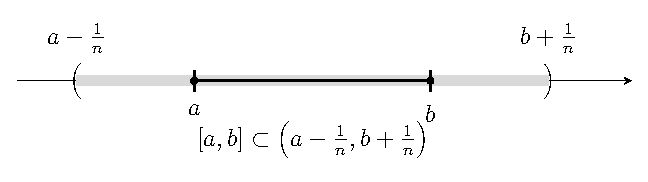
\includegraphics[width=0.82\textwidth]{aproksymacja-przedzialu.pdf}
  \caption{Przedział domknięty jako przekrój malejących przedziałów otwartych.}
  \label{fig:aproksymacja-przedzialu}
\end{figure}

\emph{Przedziały domknięte.}
Z inkluzji $\mathcal{J}_D\subseteq\mathcal{J}$ wynika
$\sigma(\mathcal{J}_D)\subseteq\mathcal{B}(\R)$.
Dla $a<b$ wybierzmy $n_0\in\N$ tak duże, aby $2/n_0<b-a$.
Wówczas
\begin{equation}
  (a,b)=\bigcup_{n=n_0}^{\infty}
    \left[a+\frac1n,b-\frac1n\right]
  \in\sigma(\mathcal{J}_D).
  \label{eq:przedzial-otwarty-suma-domknietych}
\end{equation}
Można też skorzystać z równości
\[
  (a,b)=[a,b]\setminus\bigl(\{a\}\cup\{b\}\bigr),
  \qquad \{a\}=[a,a],\quad\{b\}=[b,b].
\]
Stąd $\mathcal{J}_0\subseteq\sigma(\mathcal{J}_D)$, a więc
$\mathcal{B}(\R)\subseteq\sigma(\mathcal{J}_D)$.

\emph{Przedziały półotwarte.}
Inkluzja $\mathcal{J}_P\subseteq\mathcal{J}$ daje
$\sigma(\mathcal{J}_P)\subseteq\mathcal{B}(\R)$.
Dla $a<b$ i dostatecznie dużego $n_0$ mamy
\[
  (a,b)=\bigcup_{n=n_0}^{\infty}
    \left(a,b-\frac1n\right]\in\sigma(\mathcal{J}_P).
\]
Otrzymujemy przeciwną inkluzję, zatem
$\sigma(\mathcal{J}_P)=\mathcal{B}(\R)$.

\emph{Półproste otwarte.}
Każda półprosta $(-\infty,b)$ należy do $\mathcal{B}(\R)$, ponieważ
\[
  (-\infty,b)=\bigcup_{n=n_0}^{\infty}(-n,b)
\]
dla $n_0$ tak dużego, aby $-n_0<b$.
Stąd $\sigma(\mathcal{P}_0^-)\subseteq\mathcal{B}(\R)$.
Aby uzyskać przeciwną inkluzję, zauważmy, że
\[
  (a,+\infty)=(-\infty,a]^c
    =\left(\bigcap_{n=1}^{\infty}
      \left(-\infty,a+\frac1n\right)\right)^c
    \in\sigma(\mathcal{P}_0^-).
\]
Zatem
\[
  (a,b)=(-\infty,b)\cap(a,+\infty)
    \in\sigma(\mathcal{P}_0^-).
\]
To daje $\mathcal{J}_0\subseteq\sigma(\mathcal{P}_0^-)$ i w konsekwencji
$\mathcal{B}(\R)=\sigma(\mathcal{P}_0^-)$.
Analogicznie dla prawych półprostych korzystamy z równości
\[
  (-\infty,b)=
    \left(\bigcap_{n=1}^{\infty}
      \left(b-\frac1n,+\infty\right)\right)^c
\]
oraz $(a,b)=(a,+\infty)\cap(-\infty,b)$.
Otrzymujemy $\mathcal{B}(\R)=\sigma(\mathcal{P}_0^+)$.

\emph{Półproste domknięte.}
Pozostałe równości wynikają w ten sam sposób z zależności
\begin{align*}
  (-\infty,b]&=\bigcap_{n=1}^{\infty}
    \left(-\infty,b+\frac1n\right),
  &(-\infty,b)&=\bigcup_{n=1}^{\infty}
    \left(-\infty,b-\frac1n\right],\\
  [a,+\infty)&=\bigcap_{n=1}^{\infty}
    \left(a-\frac1n,+\infty\right),
  &(a,+\infty)&=\bigcup_{n=1}^{\infty}
    \left[a+\frac1n,+\infty\right).
\end{align*}
Rodziny półprostych otwartych i domkniętych generują więc te same sigma-ciała.
\end{proof}

\begin{uwaga}[Zbiory borelowskie w $\R^d$]
W przestrzeni $\R^d$ można zdefiniować sigma-ciało borelowskie jako
sigma-ciało generowane przez prostokąty
\[
  I_1\times\cdots\times I_d,
\]
gdzie $I_1,\ldots,I_d$ są przedziałami w $\R$.
\end{uwaga}

\section{Zbiory otwarte i sigma-ciało borelowskie}
\label{sec:otwarte-borelowskie}

\begin{definicja}[Zbiór otwarty na prostej]
Zbiór $U\subseteq\R$ nazywamy otwartym, jeżeli
\[
  \forall x\in U\ \exists\delta>0\qquad (x-\delta,x+\delta)\subseteq U.
\]
\end{definicja}

\begin{figure}[htbp]
  \centering
  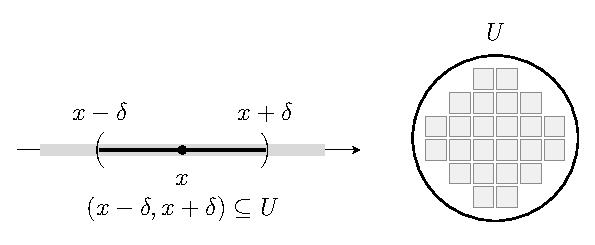
\includegraphics[width=0.91\textwidth]{otoczenie-punktu.pdf}
  \caption{Otoczenie punktu zbioru otwartego oraz prostokąty wewnątrz koła.}
  \label{fig:otoczenie-punktu}
\end{figure}

\begin{twierdzenie}
\label{tw:borelowskie-otwarte}
Niech $\tau$ będzie rodziną wszystkich zbiorów otwartych w $\R$.
Wówczas
\[
  \mathcal{B}(\R)=\sigma(\tau).
\]
\end{twierdzenie}

\begin{proof}
Każdy przedział otwarty jest zbiorem otwartym, więc
$\mathcal{B}(\R)=\sigma(\mathcal{J}_0)\subseteq\sigma(\tau)$.
Z drugiej strony każdy zbiór otwarty $U$ jest sumą zawartych w nim
przedziałów o wymiernych końcach. Jest ich co najwyżej przeliczalnie wiele,
jak w dowodzie \eqref{eq:borel-odcinki}. Zatem $\tau\subseteq\mathcal{B}(\R)$,
co daje przeciwną inkluzję.
\end{proof}

\begin{uwaga}
W przestrzeniach metrycznych, a ogólniej topologicznych, sigma-ciało
borelowskie definiuje się jako sigma-ciało generowane przez zbiory otwarte.
\end{uwaga}

\chapter{Miara}
\label{chap:miara}

\section{Funkcje zbioru i addytywność}
\label{sec:funkcje-zbioru-addytywnosc}

\begin{definicja}[Funkcja zbioru]
Niech $\mathcal{A}\subseteq\mathcal{P}(X)$ będzie rodziną zbiorów.
Odwzorowanie
\[
  \mu:\mathcal{A}\longrightarrow[0,+\infty]
\]
nazywamy funkcją zbioru.
\end{definicja}

\begin{definicja}[Skończona addytywność]
Funkcja zbioru $\mu:\mathcal{A}\to[0,+\infty]$ jest skończenie
addytywna, jeżeli dla $A,B\in\mathcal{A}$ takich, że
$A\cap B=\varnothing$ i $A\cup B\in\mathcal{A}$, zachodzi
\begin{equation}
  \mu(A\cup B)=\mu(A)+\mu(B).
  \label{eq:skonczona-addytywnosc}
\end{equation}
\end{definicja}

\begin{definicja}[Przeliczalna addytywność]
\label{def:przeliczalna-addytywnosc}
Funkcja zbioru $\mu:\mathcal{A}\to[0,+\infty]$ jest przeliczalnie
addytywna, jeżeli dla każdego ciągu parami rozłącznych zbiorów
$A_n\in\mathcal{A}$, którego suma należy do $\mathcal{A}$, mamy
\begin{equation}
  \mu\left(\bigcup_{n=1}^{\infty}A_n\right)
  =\sum_{n=1}^{\infty}\mu(A_n).
  \label{eq:przeliczalna-addytywnosc}
\end{equation}
Parami rozłączne oznacza, że $A_n\cap A_m=\varnothing$ dla $n\neq m$.
\end{definicja}

\section{Miara i przestrzeń z miarą}
\label{sec:miara-przestrzen}

\begin{definicja}[Miara]
\label{def:miara}
Niech $(X,\mathcal{F})$ będzie przestrzenią mierzalną.
Miarą na sigma-ciele $\mathcal{F}$ nazywamy przeliczalnie addytywną
funkcję zbioru
\[
  \mu:\mathcal{F}\longrightarrow[0,+\infty]
\]
spełniającą warunek $\mu(\varnothing)=0$.
\end{definicja}

\begin{definicja}[Przestrzeń z miarą]
Trójkę $(X,\mathcal{F},\mu)$, gdzie $\mathcal{F}$ jest sigma-ciałem
podzbiorów $X$, a $\mu$ jest miarą na $\mathcal{F}$,
nazywamy przestrzenią z miarą lub przestrzenią miarową.
Zbiory należące do $\mathcal{F}$ nazywamy zbiorami mierzalnymi.
\end{definicja}

\section{Własności miary}
\label{sec:wlasnosci-miary}

W tej części $(X,\mathcal{F},\mu)$ jest przestrzenią z miarą,
a wszystkie rozważane zbiory należą do $\mathcal{F}$.

\begin{fakt}[Skończona addytywność miary]
\label{fakt:miara-skonczona-addytywnosc}
Miara jest skończenie addytywna: jeżeli $A\cap B=\varnothing$, to
\[
  \mu(A\cup B)=\mu(A)+\mu(B).
\]
\end{fakt}

\begin{proof}
Połóżmy $A_1=A$, $A_2=B$ oraz $A_n=\varnothing$ dla $n\geq3$.
Zbiory tego ciągu są parami rozłączne. Z przeliczalnej addytywności
i warunku $\mu(\varnothing)=0$ otrzymujemy
\[
  \mu(A\cup B)
  =\mu\left(\bigcup_{n=1}^{\infty}A_n\right)
  =\sum_{n=1}^{\infty}\mu(A_n)=\mu(A)+\mu(B).
\]
\end{proof}

\begin{uwaga}
Indukcyjnie dla dowolnych parami rozłącznych zbiorów
$A_1,\ldots,A_n\in\mathcal{F}$ mamy
\[
  \mu\left(\bigcup_{k=1}^{n}A_k\right)=\sum_{k=1}^{n}\mu(A_k).
\]
\end{uwaga}

\begin{fakt}[Subtraktywność]
\label{fakt:miara-subtraktywnosc}
Jeżeli $A\subseteq B$ i $\mu(A)<+\infty$, to
\begin{equation}
  \mu(B\setminus A)=\mu(B)-\mu(A).
  \label{eq:miara-subtraktywnosc}
\end{equation}
\end{fakt}

\begin{proof}
Zbiory $A$ i $B\setminus A$ są mierzalne i rozłączne, a ich suma
jest równa $B$. Z faktu~\ref{fakt:miara-skonczona-addytywnosc} wynika
\begin{equation}
  \mu(B)=\mu(A)+\mu(B\setminus A).
  \label{eq:miara-rozklad-roznicy}
\end{equation}
Ponieważ $\mu(A)$ jest skończona, możemy ją odjąć i otrzymujemy
\eqref{eq:miara-subtraktywnosc}.
\end{proof}

\begin{fakt}[Miara sumy i przekroju]
\label{fakt:miara-suma-przekroj}
Dla dowolnych $A,B\in\mathcal{F}$ zachodzi
\begin{equation}
  \mu(A)+\mu(B)=\mu(A\cup B)+\mu(A\cap B).
  \label{eq:miara-suma-przekroj}
\end{equation}
\end{fakt}

\begin{proof}
Z rozkładu $A=(A\cap B)\cup(A\setminus B)$ na zbiory rozłączne
otrzymujemy
\begin{align*}
  \mu(A)+\mu(B)
    &=\mu(A\cap B)+\mu(A\setminus B)+\mu(B)\\
    &=\mu(A\cap B)+\mu\bigl((A\setminus B)\cup B\bigr)\\
    &=\mu(A\cap B)+\mu(A\cup B).
\end{align*}
W drugim przejściu użyliśmy rozłączności $A\setminus B$ i $B$.
\end{proof}

\begin{fakt}[Monotoniczność]
\label{fakt:miara-monotonicznosc}
Jeżeli $A\subseteq B$, to $\mu(A)\leq\mu(B)$.
\end{fakt}

\begin{proof}
Z równości~\eqref{eq:miara-rozklad-roznicy} i nieujemności miary wynika
\[
  \mu(B)=\mu(A)+\mu(B\setminus A)\geq\mu(A).
\]
Sam rozkład~\eqref{eq:miara-rozklad-roznicy} nie wymaga założenia
o skończoności $\mu(A)$.
\end{proof}

\begin{fakt}[Przeliczalna podaddytywność]
\label{fakt:miara-podaddytywnosc}
Dla dowolnego ciągu zbiorów $A_n\in\mathcal{F}$ zachodzi
\begin{equation}
  \mu\left(\bigcup_{n=1}^{\infty}A_n\right)
  \leq\sum_{n=1}^{\infty}\mu(A_n).
  \label{eq:miara-podaddytywnosc}
\end{equation}
\end{fakt}

\begin{proof}
Połóżmy $B_1=A_1$ oraz dla $n\geq1$
\begin{equation}
  B_{n+1}=A_{n+1}\setminus\bigcup_{k=1}^{n}A_k.
  \label{eq:rozlacznienie-ciagu}
\end{equation}
Zbiory $B_n$ są mierzalne, parami rozłączne i spełniają $B_n\subseteq A_n$.
Ponadto
\[
  \bigcup_{n=1}^{\infty}B_n=\bigcup_{n=1}^{\infty}A_n:
\]
każdy punkt sumy należy do pierwszego zbioru $A_n$, w którym się pojawia,
a więc należy do odpowiedniego $B_n$.
Z przeliczalnej addytywności i monotoniczności miary otrzymujemy
\[
  \mu\left(\bigcup_{n=1}^{\infty}A_n\right)
  =\mu\left(\bigcup_{n=1}^{\infty}B_n\right)
  =\sum_{n=1}^{\infty}\mu(B_n)
  \leq\sum_{n=1}^{\infty}\mu(A_n).
\]
\end{proof}

\begin{figure}[htbp]
  \centering
  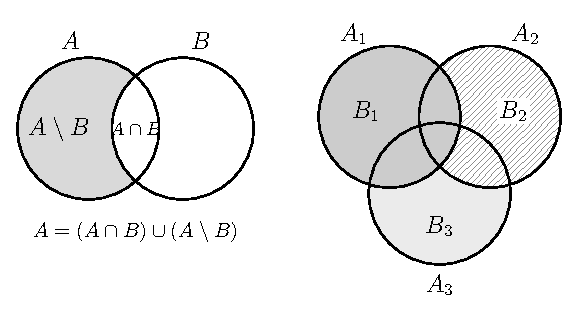
\includegraphics[width=0.93\textwidth]{roznica-i-rozlacznienie.pdf}
  \caption{Rozkład zbioru $A$ oraz rozłącznienie pierwszych trzech zbiorów ciągu.}
  \label{fig:roznica-i-rozlacznienie}
\end{figure}

% Zamknij rysunki poprzedniego wykładu przed nowym znacznikiem i sekcją.
\clearpage
\poczatekwykladu{5}
\section{Ciągłość miary}
\label{sec:ciaglosc-miary}

Niech $(X,\mathcal{F},\mu)$ będzie przestrzenią z miarą.

\begin{fakt}[Ciągłość z dołu]
\label{fakt:ciaglosc-z-dolu}
Jeżeli $A_n\in\mathcal{F}$ i $A_1\subseteq A_2\subseteq\cdots$, to
\begin{equation}
  \lim_{n\to\infty}\mu(A_n)
  =\mu\left(\bigcup_{n=1}^{\infty}A_n\right)
  =\mu\left(\lim_{n\to\infty}A_n\right).
  \label{eq:ciaglosc-z-dolu}
\end{equation}
Własność tę nazywamy również ciągłością miary w górę.
\end{fakt}

\begin{proof}
Połóżmy $A_0=\varnothing$ i $B_n=A_n\setminus A_{n-1}$ dla $n\geq1$.
Zbiory $B_n$ są mierzalne i parami rozłączne, a ponadto
\[
  \bigcup_{n=1}^{\infty}B_n=\bigcup_{n=1}^{\infty}A_n,
  \qquad \bigcup_{n=1}^{N}B_n=A_N.
\]
Z przeliczalnej i skończonej addytywności otrzymujemy
\begin{align*}
  \mu\left(\bigcup_{n=1}^{\infty}A_n\right)
    &=\mu\left(\bigcup_{n=1}^{\infty}B_n\right)
      =\sum_{n=1}^{\infty}\mu(B_n)\\
    &=\lim_{N\to\infty}\sum_{n=1}^{N}\mu(B_n)
      =\lim_{N\to\infty}\mu\left(\bigcup_{n=1}^{N}B_n\right)\\
    &=\lim_{N\to\infty}\mu(A_N).
\end{align*}
Dla ciągu wstępującego granica zbiorów jest równa ich sumie,
co uzasadnia ostatnią równość w \eqref{eq:ciaglosc-z-dolu}.
\end{proof}

\begin{fakt}[Ciągłość z góry dla miary skończonej]
\label{fakt:ciaglosc-z-gory}
Jeżeli $\mu(X)<+\infty$, $A_n\in\mathcal{F}$ oraz
$A_1\supseteq A_2\supseteq\cdots$, to
\begin{equation}
  \lim_{n\to\infty}\mu(A_n)
  =\mu\left(\bigcap_{n=1}^{\infty}A_n\right)
  =\mu\left(\lim_{n\to\infty}A_n\right).
  \label{eq:ciaglosc-z-gory}
\end{equation}
Własność tę nazywamy również ciągłością miary w dół.
\end{fakt}

\begin{proof}
Ciąg $(A_n^c)$ jest wstępujący. Z ciągłości z dołu i praw de Morgana
otrzymujemy
\[
  \lim_{n\to\infty}\mu(A_n^c)
  =\mu\left(\bigcup_{n=1}^{\infty}A_n^c\right)
  =\mu\left(\left(\bigcap_{n=1}^{\infty}A_n\right)^c\right).
\]
Ponieważ $\mu(X)$ jest skończona, z subtraktywności wynika
$\mu(A_n)=\mu(X)-\mu(A_n^c)$.
Odejmując powyższą granicę od $\mu(X)$, dostajemy
\eqref{eq:ciaglosc-z-gory}.
\end{proof}

\section{Miary skończone, sigma-skończone i zupełne}
\label{sec:rodzaje-miar}

\begin{definicja}[Miara skończona]
Miarę $\mu$ na $(X,\mathcal{F})$ nazywamy skończoną, jeżeli
$\mu(X)<+\infty$. Równoważnie, każdy zbiór $A\in\mathcal{F}$
ma skończoną miarę. Równoważność wynika z monotoniczności
oraz z warunku $X\in\mathcal{F}$.
\end{definicja}

\begin{definicja}[Miara sigma-skończona]
Miarę $\mu$ nazywamy sigma-skończoną
($\sigma$-skończoną), jeżeli istnieją zbiory $X_n\in\mathcal{F}$ takie, że
\begin{equation}
  X=\bigcup_{n=1}^{\infty}X_n,
  \qquad \mu(X_n)<+\infty\quad\text{dla każdego }n\geq1.
  \label{eq:sigma-skonczonosc}
\end{equation}
\end{definicja}

\begin{definicja}[Miara zupełna]
Miarę $\mu$ na $(X,\mathcal{F})$ nazywamy zupełną, jeżeli każdy
podzbiór mierzalnego zbioru miary zero jest mierzalny. To znaczy:
jeżeli $A\subseteq B$, $B\in\mathcal{F}$ i $\mu(B)=0$, to
$A\in\mathcal{F}$. Wtedy również $\mu(A)=0$, na mocy monotoniczności.
\end{definicja}

\section{Przykłady miar}
\label{sec:przyklady-miar}

\begin{przyklad}[Miara licząca]
\label{prz:miara-liczaca}
Na przestrzeni mierzalnej $(X,\mathcal{P}(X))$ określamy
\begin{equation}
  \eta(A)=
  \begin{cases}
    |A|, & \text{gdy }A\text{ jest skończony},\\
    +\infty, & \text{gdy }A\text{ jest nieskończony}.
  \end{cases}
  \label{eq:miara-liczaca}
\end{equation}
Funkcja $\eta$ jest miarą, nazywaną miarą liczącą.
\end{przyklad}

\begin{proof}
Funkcja jest określona na wszystkich podzbiorach $X$, przyjmuje wartości
w $[0,+\infty]$ i spełnia $\eta(\varnothing)=0$.
Niech $A_1,A_2,\ldots$ będą parami rozłączne.

Jeżeli pewien $A_{n_0}$ jest nieskończony, to zarówno
$\eta(\bigcup_{n=1}^{\infty}A_n)$, jak i
$\sum_{n=1}^{\infty}\eta(A_n)$ są równe $+\infty$.

Załóżmy teraz, że wszystkie $A_n$ są skończone.
Jeżeli ich suma jest skończona, to tylko skończenie wiele z nich
jest niepustych. Dla pewnego $N$ mamy więc
\[
  \eta\left(\bigcup_{n=1}^{\infty}A_n\right)
  =\left|\bigcup_{n=1}^{N}A_n\right|
  =\sum_{n=1}^{N}|A_n|
  =\sum_{n=1}^{\infty}\eta(A_n).
\]
Jeżeli ich suma jest nieskończona, to nieskończenie wiele zbiorów $A_n$
jest niepustych. Każdy z nich ma co najmniej jeden element, zatem
\[
  \sum_{n=1}^{\infty}\eta(A_n)=+\infty
  =\eta\left(\bigcup_{n=1}^{\infty}A_n\right).
\]
We wszystkich przypadkach zachodzi przeliczalna addytywność.
\end{proof}

\begin{przyklad}[Miara skupiona w jednym punkcie]
\label{prz:dirac}
Ustalmy $x\in X$. Na $(X,\mathcal{P}(X))$ określamy
\begin{equation}
  \delta_x(A)=
  \begin{cases}
    1, & \text{gdy }x\in A,\\
    0, & \text{gdy }x\notin A.
  \end{cases}
  \label{eq:dirac}
\end{equation}
Jest to miara skupiona w punkcie $x$, zwana miarą Diraca
lub deltą Diraca. Można ją zapisać również jako $\delta_x(A)=\mathbf{1}_A(x)$.
\end{przyklad}

\begin{proof}
Mamy $\delta_x(\varnothing)=0$.
Jeżeli $A_n$ są parami rozłączne, to punkt $x$ należy do co najwyżej
jednego z nich. Gdy nie należy do żadnego, obie strony równości
addytywności są równe zero; gdy należy do jednego, obie są równe jeden.
Zatem $\delta_x$ jest przeliczalnie addytywna.
\end{proof}

\begin{przyklad}[Miara o skończonym nośniku]
\label{prz:skonczony-nosnik}
Niech $x_1,\ldots,x_N\in X$ oraz niech $a_1,\ldots,a_N\in[0,+\infty]$
będą ustalonymi wagami. Wtedy wzór
\begin{equation}
  \mu(A)=\sum_{n=1}^{N}a_n\delta_{x_n}(A),
  \qquad A\subseteq X,
  \label{eq:miara-skonczony-nosnik}
\end{equation}
określa miarę na $(X,\mathcal{P}(X))$.
Przy wagach nieskończonych stosujemy przyjętą wcześniej konwencję
$0\cdot(+\infty)=0$.
\end{przyklad}

\begin{proof}
Każdy składnik jest nieujemny i dla $A=\varnothing$ ma wartość zero.
Dla parami rozłącznych zbiorów $A_k$ mamy
\begin{align*}
  \mu\left(\bigcup_{k=1}^{\infty}A_k\right)
    &=\sum_{n=1}^{N}a_n
      \delta_{x_n}\left(\bigcup_{k=1}^{\infty}A_k\right)\\
    &=\sum_{n=1}^{N}\sum_{k=1}^{\infty}a_n\delta_{x_n}(A_k)\\
    &=\sum_{k=1}^{\infty}\sum_{n=1}^{N}a_n\delta_{x_n}(A_k)
      =\sum_{k=1}^{\infty}\mu(A_k).
\end{align*}
Wykorzystaliśmy addytywność miar Diraca i możliwość zamiany kolejności
sumowania wyrazów nieujemnych. Dla ustalonego $n$ tylko jeden z wyrazów
$\delta_{x_n}(A_k)$ może być niezerowy, co uzasadnia rachunek także
przy $a_n=+\infty$.
\end{proof}

\begin{figure}[htbp]
  \centering
  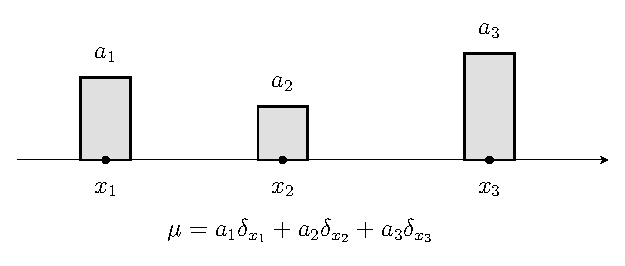
\includegraphics[width=0.76\textwidth]{miara-punktowa.pdf}
  \caption{Skończenie wiele punktów z przypisanymi wagami.}
  \label{fig:miara-punktowa}
\end{figure}

\section{Miara zewnętrzna Lebesgue'a}
\label{sec:miara-zewnetrzna-lebesgue}

\begin{definicja}[Miara zewnętrzna Lebesgue'a na prostej]
\label{def:miara-zewnetrzna-lebesgue}
Dla dowolnego $A\subseteq\R$ określamy
\begin{equation}
  \lambda^{\ast}(A)=\inf\left\{
    \sum_{n=1}^{\infty}|I_n|:
    A\subseteq\bigcup_{n=1}^{\infty}I_n,
    \ I_n\text{ są przedziałami}\right\}.
  \label{eq:miara-zewnetrzna-lebesgue}
\end{equation}
Symbol $|I_n|$ oznacza tu długość przedziału $I_n$.
Dla przedziału ograniczonego o końcach $a\leq b$ jest ona równa $b-a$,
niezależnie od uwzględnienia końców; przedziały nieograniczone mają
długość $+\infty$. Dopuszczamy przedziały jednopunktowe długości zero.
\end{definicja}

\begin{fakt}[Nieujemność i wartość na zbiorze pustym]
\label{fakt:zewnetrzna-zero}
Dla każdego $A\subseteq\R$ mamy $\lambda^{\ast}(A)\geq0$, a ponadto
$\lambda^{\ast}(\varnothing)=0$.
\end{fakt}

\begin{proof}
Każda suma długości przedziałów jest nieujemna, więc jej infimum
jest nieujemne. Zbiór pusty można pokryć ciągiem przedziałów
$I_n=[0,0]$; suma ich długości wynosi zero.
\end{proof}

\begin{fakt}[Monotoniczność miary zewnętrznej]
\label{fakt:zewnetrzna-monotonicznosc}
Jeżeli $A\subseteq B\subseteq\R$, to
$\lambda^{\ast}(A)\leq\lambda^{\ast}(B)$.
\end{fakt}

\begin{proof}
Każde pokrycie $B$ przedziałami pokrywa również $A$.
Zbiór dopuszczalnych sum długości dla $A$ zawiera więc zbiór
dopuszczalnych sum długości dla $B$. Przejście do infimów daje
żądaną nierówność.
\end{proof}

\begin{fakt}[Przeliczalna podaddytywność miary zewnętrznej]
\label{fakt:zewnetrzna-podaddytywnosc}
Dla dowolnych zbiorów $A_n\subseteq\R$ zachodzi
\begin{equation}
  \lambda^{\ast}\left(\bigcup_{n=1}^{\infty}A_n\right)
  \leq\sum_{n=1}^{\infty}\lambda^{\ast}(A_n).
  \label{eq:zewnetrzna-podaddytywnosc}
\end{equation}
\end{fakt}

\begin{proof}
Jeżeli suma po prawej stronie jest nieskończona, nierówność jest oczywista.
Załóżmy więc, że jest skończona, i ustalmy $\varepsilon>0$.
Dla każdego $n\geq1$ wybieramy pokrycie $A_n$ przedziałami
$I_1^{(n)},I_2^{(n)},\ldots$ takie, że
\[
  \sum_{k=1}^{\infty}|I_k^{(n)}|
  <\lambda^{\ast}(A_n)+\frac{\varepsilon}{2^n}.
\]
Możemy to zrobić z definicji infimum.
Rodzina $\{I_k^{(n)}:n,k\in\N\}$ jest przeliczalna i pokrywa
$\bigcup_{n=1}^{\infty}A_n$. Zatem
\begin{align*}
  \lambda^{\ast}\left(\bigcup_{n=1}^{\infty}A_n\right)
    &\leq\sum_{n=1}^{\infty}\sum_{k=1}^{\infty}|I_k^{(n)}|\\
    &\leq\sum_{n=1}^{\infty}
      \left(\lambda^{\ast}(A_n)+\frac{\varepsilon}{2^n}\right)\\
    &=\sum_{n=1}^{\infty}\lambda^{\ast}(A_n)+\varepsilon.
\end{align*}
Z dowolności $\varepsilon>0$ otrzymujemy
\eqref{eq:zewnetrzna-podaddytywnosc}.
\end{proof}

\section{Miary zewnętrzne}
\label{sec:miary-zewnetrzne}

\begin{uwaga}[Rodzaje przedziałów w pokryciach]
\label{uw:rodzaje-pokryc}
W definicji~\ref{def:miara-zewnetrzna-lebesgue} otrzymamy tę samą
wartość $\lambda^{\ast}(A)$, jeżeli dopuścimy wyłącznie przedziały
otwarte albo wyłącznie przedziały domknięte. Możemy też dopuścić
zbiór pusty, przyjmując $|\varnothing|=0$.
\end{uwaga}

\begin{proof}
Ograniczenie rodziny dopuszczalnych pokryć może tylko zwiększyć infimum.
Jeżeli $\lambda^{\ast}(A)=+\infty$, wszystkie rozważane infima są więc
równe $+\infty$. W przeciwnym przypadku ustalmy $\varepsilon>0$
i wybierzmy pokrycie $A$ przedziałami $I_n$ takie, że
\[
  \sum_{n=1}^{\infty}|I_n|<\lambda^{\ast}(A)+\varepsilon.
\]
Każdy $I_n$ ma skończoną długość. Możemy go zawrzeć w przedziale
otwartym $J_n$ o długości mniejszej niż $|I_n|+\varepsilon/2^n$.
Wtedy $J_n$ pokrywają $A$ i
\[
  \sum_{n=1}^{\infty}|J_n|<\lambda^{\ast}(A)+2\varepsilon.
\]
Infimum dla pokryć otwartych jest zatem równe $\lambda^{\ast}(A)$.
Zastąpienie każdego $I_n$ jego domknięciem nie zmienia długości,
więc równość zachodzi również dla pokryć domkniętych.
Puste składniki pokrycia można zastąpić przedziałami jednopunktowymi
długości zero; ich dopuszczenie także nie zmienia infimum.
\end{proof}

\begin{samepage}
\begin{definicja}[Miara zewnętrzna]
\label{def:miara-zewnetrzna}
Miarą zewnętrzną na zbiorze $X$ nazywamy funkcję zbioru
$\mu^{\ast}\colon\mathcal{P}(X)\to[0,+\infty]$, która spełnia warunki:
\begin{enumerate}
  \item $\mu^{\ast}(\varnothing)=0$;
  \item jeżeli $A\subseteq B\subseteq X$, to
    $\mu^{\ast}(A)\leq\mu^{\ast}(B)$;
  \item dla dowolnych $A_n\subseteq X$ zachodzi
    \[
      \mu^{\ast}\left(\bigcup_{n=1}^{\infty}A_n\right)
      \leq\sum_{n=1}^{\infty}\mu^{\ast}(A_n).
    \]
\end{enumerate}
Są to kolejno: zerowanie na zbiorze pustym, monotoniczność
i przeliczalna podaddytywność.
\end{definicja}
\end{samepage}

\begin{uwaga}
Funkcja $\lambda^{\ast}$ jest miarą zewnętrzną na $\R$, zgodnie
z faktami~\ref{fakt:zewnetrzna-zero}--\ref{fakt:zewnetrzna-podaddytywnosc}.
Miara zewnętrzna może przyjmować wartość $+\infty$.
\end{uwaga}

\section{Warunek mierzalności Carathéodory'ego}
\label{sec:caratheodory}

\begin{definicja}[Zbiór mierzalny względem miary zewnętrznej]
\label{def:caratheodory}
Niech $\mu^{\ast}$ będzie miarą zewnętrzną na $X$.
Zbiór $E\subseteq X$ nazywamy $\mu^{\ast}$-mierzalnym, jeżeli
dla każdego zbioru $A\subseteq X$ zachodzi
\begin{equation}
  \mu^{\ast}(A)
  =\mu^{\ast}(A\cap E)+\mu^{\ast}(A\cap E^c).
  \label{eq:caratheodory}
\end{equation}
Dopełnienie $E^c$ jest brane względem $X$.
Równość~\eqref{eq:caratheodory} nazywamy warunkiem mierzalności
Carathéodory'ego.
\end{definicja}

\begin{twierdzenie}[Carathéodory'ego]
\label{tw:caratheodory}
Rodzina $\mathcal{F}$ wszystkich zbiorów $\mu^{\ast}$-mierzalnych
jest sigma-ciałem. Obcięcie
\[
  \mu=\mu^{\ast}|_{\mathcal{F}}
  \colon\mathcal{F}\longrightarrow[0,+\infty]
\]
jest miarą zupełną.
\end{twierdzenie}

\begin{proof}
\emph{Sigma-ciało.}
Zbiór pusty jest mierzalny, bo
$\mu^{\ast}(A\cap\varnothing)+\mu^{\ast}(A\cap X)=\mu^{\ast}(A)$.
Warunek~\eqref{eq:caratheodory} jest symetryczny względem $E$ i $E^c$,
więc $\mathcal{F}$ jest zamknięta na dopełnienia.

Niech $E,F\in\mathcal{F}$. Dzieląc najpierw $A$ przez $E$, a potem
$A\cap E^c$ przez $F$, otrzymujemy
\begin{align*}
  \mu^{\ast}(A)
    &=\mu^{\ast}(A\cap E)+\mu^{\ast}(A\cap E^c\cap F)
      +\mu^{\ast}(A\cap E^c\cap F^c)\\
    &\geq\mu^{\ast}\bigl(A\cap(E\cup F)\bigr)
      +\mu^{\ast}\bigl(A\cap(E\cup F)^c\bigr).
\end{align*}
W nierówności zastosowaliśmy podaddytywność do dwóch pierwszych
składników. Przeciwna nierówność również wynika z podaddytywności,
zatem $E\cup F\in\mathcal{F}$.

Niech teraz $E_n\in\mathcal{F}$ będą parami rozłączne, a
$S_N=\bigcup_{n=1}^{N}E_n$ i $S=\bigcup_{n=1}^{\infty}E_n$.
Kolejne zastosowania warunku mierzalności dają
\[
  \mu^{\ast}(A)
  =\sum_{n=1}^{N}\mu^{\ast}(A\cap E_n)+\mu^{\ast}(A\setminus S_N)
  \geq\sum_{n=1}^{N}\mu^{\ast}(A\cap E_n)
      +\mu^{\ast}(A\setminus S).
\]
Przechodząc z $N$ do nieskończoności i stosując podaddytywność,
otrzymujemy
\[
  \mu^{\ast}(A)
  \geq\sum_{n=1}^{\infty}\mu^{\ast}(A\cap E_n)
       +\mu^{\ast}(A\setminus S)
  \geq\mu^{\ast}(A\cap S)+\mu^{\ast}(A\cap S^c).
\]
Przeciwna nierówność jest automatyczna, więc $S\in\mathcal{F}$.
Dla dowolnego ciągu $F_n\in\mathcal{F}$ stosujemy rozłącznienie
\[
  E_1=F_1,\qquad
  E_n=F_n\setminus\bigcup_{k=1}^{n-1}F_k\quad(n\geq2).
\]
Zamknięcie na dopełnienia i skończone sumy zapewnia $E_n\in\mathcal{F}$,
a równość sum obu ciągów daje $\bigcup_nF_n\in\mathcal{F}$.
Zatem $\mathcal{F}$ jest sigma-ciałem.

\emph{Miara.}
Mamy $\mu(\varnothing)=0$.
Dla rozłącznych $E,F\in\mathcal{F}$, stosując mierzalność $F$ do
$A=E\cup F$, otrzymujemy
\[
  \mu(E\cup F)
  =\mu^{\ast}\bigl((E\cup F)\cap F\bigr)
   +\mu^{\ast}\bigl((E\cup F)\cap F^c\bigr)
  =\mu(F)+\mu(E).
\]
Indukcyjnie dostajemy addytywność dla dowolnej skończonej rodziny.
Dla parami rozłącznych $E_n\in\mathcal{F}$ monotoniczność daje
\[
  \mu\left(\bigcup_{n=1}^{\infty}E_n\right)
  \geq\mu\left(\bigcup_{n=1}^{N}E_n\right)
  =\sum_{n=1}^{N}\mu(E_n).
\]
Po przejściu do granicy otrzymujemy nierówność z sumą nieskończoną.
Nierówność przeciwna wynika z podaddytywności $\mu^{\ast}$,
co dowodzi przeliczalnej addytywności $\mu$.

\emph{Zupełność.}
Niech $Z\subseteq B$, gdzie $B\in\mathcal{F}$ i $\mu(B)=0$.
Z monotoniczności $\mu^{\ast}(Z)=0$, więc dla każdego $A\subseteq X$
mamy $\mu^{\ast}(A\cap Z)=0$ oraz
\[
  \mu^{\ast}(A\cap Z)+\mu^{\ast}(A\cap Z^c)
  =\mu^{\ast}(A\cap Z^c)\leq\mu^{\ast}(A).
\]
Przeciwna nierówność wynika z podaddytywności.
Zatem $Z$ jest mierzalny, czyli $Z\in\mathcal{F}$.
\end{proof}

\begin{wniosek}[Miara Lebesgue'a]
\label{wn:miara-lebesgue}
Niech $\mathcal{L}$ oznacza rodzinę wszystkich
$\lambda^{\ast}$-mierzalnych podzbiorów $\R$. Wówczas
\[
  \lambda=\lambda^{\ast}|_{\mathcal{L}}
\]
jest miarą zupełną, a $(\R,\mathcal{L},\lambda)$ jest zupełną
przestrzenią z miarą. Miarę $\lambda$ nazywamy miarą Lebesgue'a,
a $\mathcal{L}$ --- sigma-ciałem zbiorów mierzalnych w sensie Lebesgue'a.
\end{wniosek}

\begin{uwaga}
Zbiór Vitaliego $V$ z przykładu~\ref{prz:vitali} nie należy do
$\mathcal{L}$. Gdyby był mierzalny, mierzalne byłyby też jego
przesunięcia (jak wykażemy poniżej), a addytywność $\lambda$
prowadziłaby do otrzymanej tam sprzeczności.
\end{uwaga}

\section{Własności miary Lebesgue'a}
\label{sec:wlasnosci-lebesgue}

\begin{samepage}
\begin{fakt}
\label{fakt:wlasnosci-lebesgue}
Miara Lebesgue'a i jej miara zewnętrzna mają następujące własności:
\begin{enumerate}
  \item Jeżeli $E\in\mathcal{L}$ i $x\in\R$, to $E+x\in\mathcal{L}$
    i $\lambda(E+x)=\lambda(E)$.
  \item Każdy zbiór przeliczalny $F\subseteq\R$ należy do
    $\mathcal{L}$ i ma miarę zero. W szczególności
    $\lambda(\{x\})=0$ dla $x\in\R$.
  \item Dla każdego przedziału $I\subseteq\R$ zachodzi
    $\lambda^{\ast}(I)=|I|$.
  \item Każda półprosta $(-\infty,b)$, gdzie $b\in\R$,
    należy do $\mathcal{L}$.
  \item $\mathcal{B}(\R)\subseteq\mathcal{L}$.
\end{enumerate}
\end{fakt}
\end{samepage}

\begin{proof}
\emph{Ad 1.}
Niech $E\in\mathcal{L}$. Dla dowolnego $A\subseteq\R$ stosujemy
mierzalność $E$ do $A-x$. Z niezmienniczości $\lambda^{\ast}$
na przesunięcia wynika
\begin{align*}
  \lambda^{\ast}(A)
    &=\lambda^{\ast}(A-x)\\
    &=\lambda^{\ast}\bigl((A-x)\cap E\bigr)
      +\lambda^{\ast}\bigl((A-x)\cap E^c\bigr)\\
    &=\lambda^{\ast}\bigl(A\cap(E+x)\bigr)
      +\lambda^{\ast}\bigl(A\cap(E+x)^c\bigr).
\end{align*}
Zatem $E+x\in\mathcal{L}$ i
$\lambda(E+x)=\lambda^{\ast}(E+x)=\lambda^{\ast}(E)=\lambda(E)$.

\emph{Ad 2.}
Przedział $[x,x]$ pokrywa $\{x\}$ i ma długość zero,
więc $\lambda^{\ast}(\{x\})=0$.
Przeliczalna podaddytywność daje $\lambda^{\ast}(F)=0$
dla każdego przeliczalnego $F$.
Każdy zbiór miary zewnętrznej zero jest mierzalny:
dla dowolnego $A$ jeden składnik warunku Carathéodory'ego jest zerowy,
a drugi nie przekracza $\lambda^{\ast}(A)$; przeciwną nierówność
daje podaddytywność. Stąd $F\in\mathcal{L}$ i $\lambda(F)=0$.

\emph{Ad 3.}
Dla przedziału ograniczonego $I$ o końcach $a\leq b$ pokrycie nim samym
daje $\lambda^{\ast}(I)\leq b-a$.
Dla odcinka domkniętego $[a,b]$ powtarzamy argument
z uwagi~\ref{uw:dlugosc-przedzialu-vitali}:
dowolne pokrycie rozszerzamy do otwartego z przyrostem sumy długości
mniejszym niż $\varepsilon$, wybieramy podpokrycie skończone
i korzystamy z tego, że suma jego długości jest co najmniej $b-a$.
Z dowolności $\varepsilon>0$ wynika
$\lambda^{\ast}([a,b])\geq b-a$.

Jeżeli $a<b$, to dla $0<\delta<(b-a)/2$ odcinek
$[a+\delta,b-\delta]$ zawiera się w $I$. Monotoniczność daje
\[
  b-a-2\delta\leq\lambda^{\ast}(I)\leq b-a.
\]
Przejście z $\delta$ do zera dowodzi równości dla wszystkich rodzajów
końców. Przypadek jednopunktowy wynika z punktu 2.
Przedział nieograniczony zawiera odcinki domknięte o dowolnie dużej
długości, zatem jego miara zewnętrzna jest nieskończona.

\emph{Ad 4.}
Ustalmy $b\in\R$, $E=(-\infty,b)$ i dowolny $A\subseteq\R$.
Oznaczmy
\[
  A_1=A\cap(-\infty,b),\qquad A_2=A\cap[b,+\infty).
\]
Podaddytywność daje
$\lambda^{\ast}(A)\leq\lambda^{\ast}(A_1)+\lambda^{\ast}(A_2)$.
Wystarczy wykazać przeciwną nierówność.
Gdy $\lambda^{\ast}(A)=+\infty$, jest ona automatyczna.
Załóżmy więc, że $\lambda^{\ast}(A)<+\infty$, i ustalmy
$\varepsilon>0$. Na mocy uwagi~\ref{uw:rodzaje-pokryc} istnieje
pokrycie $A$ przedziałami otwartymi $I_n$ takie, że
\[
  \sum_{n=1}^{\infty}|I_n|<\lambda^{\ast}(A)+\varepsilon.
\]
Połóżmy
\[
  I_n^-=I_n\cap(-\infty,b),\qquad
  I_n^+=I_n\cap[b,+\infty).
\]
Są to przedziały lub zbiory puste, przy czym
$|I_n|=|I_n^-|+|I_n^+|$.
Rodziny $(I_n^-)$ i $(I_n^+)$ pokrywają odpowiednio $A_1$ i $A_2$.
W definicji miary zewnętrznej wolno użyć także tych przedziałów
i pustych składników, więc
\begin{align*}
  \lambda^{\ast}(A_1)+\lambda^{\ast}(A_2)
    &\leq\sum_{n=1}^{\infty}|I_n^-|+\sum_{n=1}^{\infty}|I_n^+|\\
    &=\sum_{n=1}^{\infty}\bigl(|I_n^-|+|I_n^+|\bigr)
      =\sum_{n=1}^{\infty}|I_n|\\
    &<\lambda^{\ast}(A)+\varepsilon.
\end{align*}
Z dowolności $\varepsilon>0$ otrzymujemy żądaną nierówność.
Zatem $E\in\mathcal{L}$.

\emph{Ad 5.}
Z twierdzenia~\ref{tw:generatory-borelowskie} i punktu 4 wynika
\[
  \mathcal{B}(\R)
  =\sigma\bigl(\{(-\infty,b):b\in\R\}\bigr)
  \subseteq\mathcal{L},
\]
ponieważ $\mathcal{L}$ jest sigma-ciałem zawierającym wszystkie
wskazane półproste.
\end{proof}


\end{document}

